\chapter{La reproducción y el entorno}\label{ch:g8:reproduction-and-environment}

¿Por qué empieza el coro de las ranas en mayo y no en noviembre? ¿Por
qué un buen año de hayas llena el bosque de \omterm{prop:g2:from-seed-to-plant:cycle}{plántulas}, y un junio frío
y lluvioso vacía de ranitas la charca de la primavera siguiente? El
capítulo anterior construyó el mecanismo de la generación siguiente;
este lo enchufa al mundo: la reproducción está marcada, abastecida ---
y limitada --- por el \omterm{def:g6:exploring-our-environment:components}{entorno}.

\section{Marcada por las estaciones}

\begin{proposition}[La cría sigue el calendario de la abundancia]\label{prop:g8:reproduction-and-environment:timing}
Las \omterm{def:g5:biodiversity:species}{especies} ajustan su reproducción para que las \emph{crías} lleguen
cuando las \omterm{def:g6:exploring-our-environment:conditions}{condiciones} y la comida les vayan a servir
(\cref{prop:g6:life-through-seasons:conditions}):
\begin{itemize}
  \item el herrerillo pone de manera que sus pollos salgan del \omterm{def:g2:animals-grow-up:born}{huevo} en
        el máximo de \omterm{ex:g2:animals-grow-up:butterfly}{orugas} de la primavera (la cadena del roble del
        \cref{ex:g3:food-chains:three}, ajustada al día);
  \item la rana desova en la charca que se templa, para darles a los
        \omterm{ex:g2:animals-grow-up:frog}{renacuajos} un verano de crecimiento antes del invierno;
  \item las \omterm{def:g1:plants-around-us:plant}{plantas} florecen en la temporada de sus polinizadores y
        maduran la \omterm{def:g2:from-seed-to-plant:seed}{semilla} según el calendario de la \omterm{def:g6:how-plants-spread:dispersal}{dispersión}
        (\cref{pb:g6:life-through-seasons:1});
  \item la berrea de otoño del ciervo coloca los partos en la
        \emph{primavera} siguiente --- con la gestación contada.
\end{itemize}
Las señales que ponen en marcha la maquinaria son las señales del
propio \omterm{def:g6:exploring-our-environment:components}{entorno}: sobre todo los días que se alargan, el calor, la lluvia.
\end{proposition}
\admitted

\begin{omfigure}
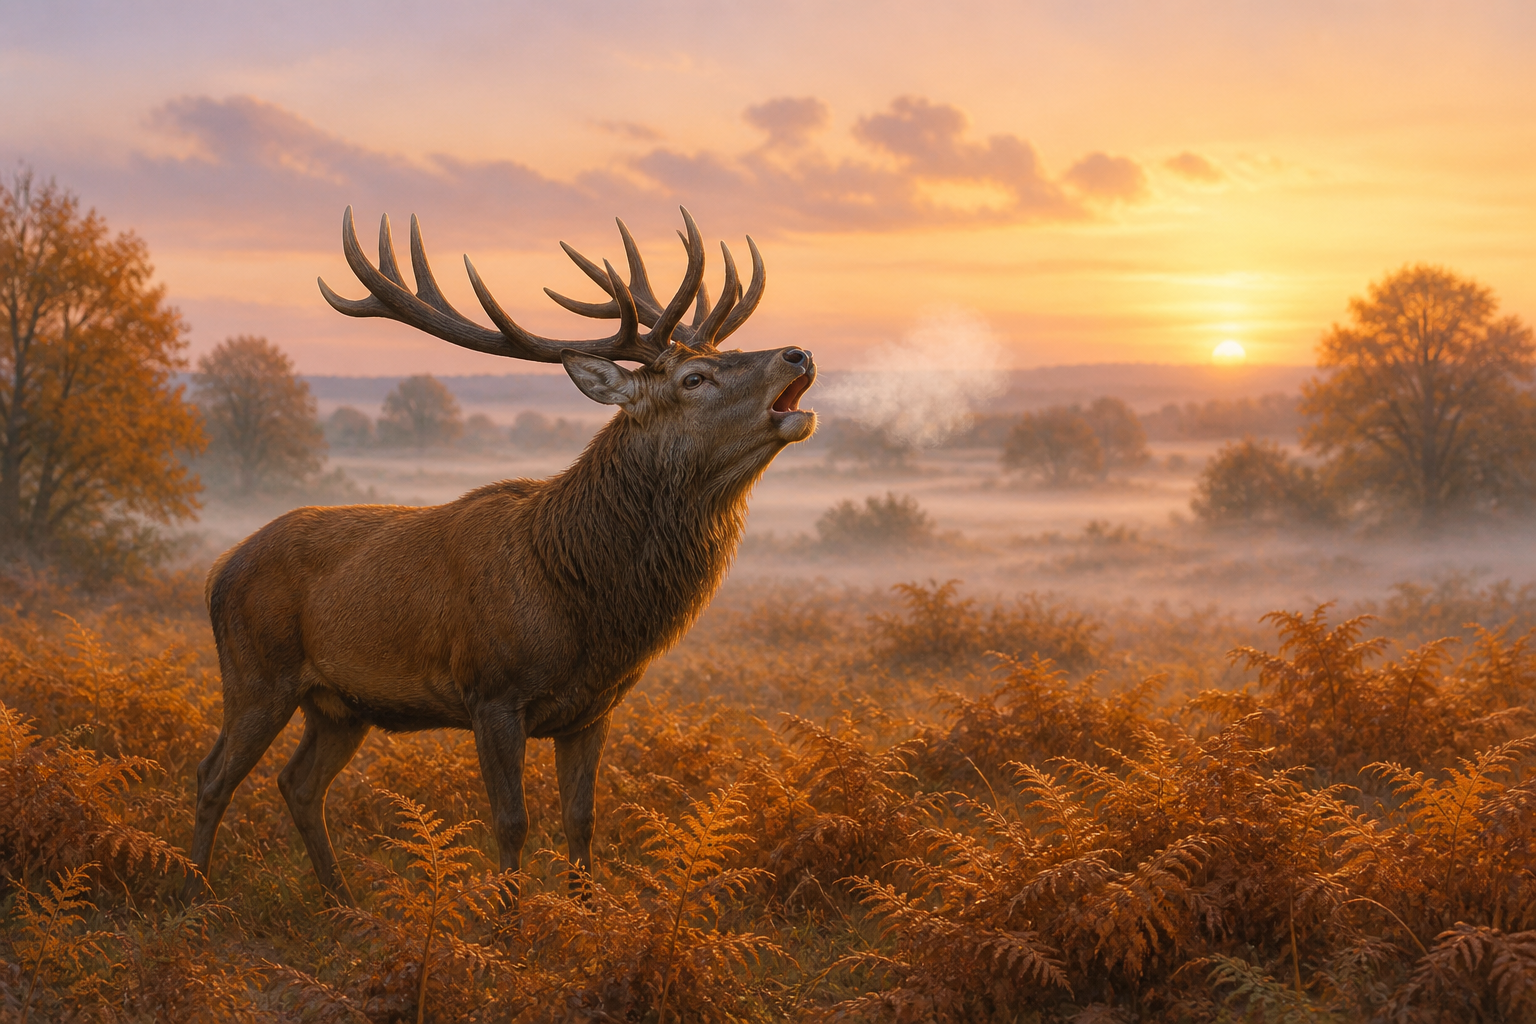
\includegraphics[width=0.6\linewidth]{images/book1/ai/g8-repro-stag.png}

{\small La berrea del otoño, la aritmética de la primavera: el ciervo
cuenta la gestación en sus fechas.}
\end{omfigure}

\begin{omfigure}
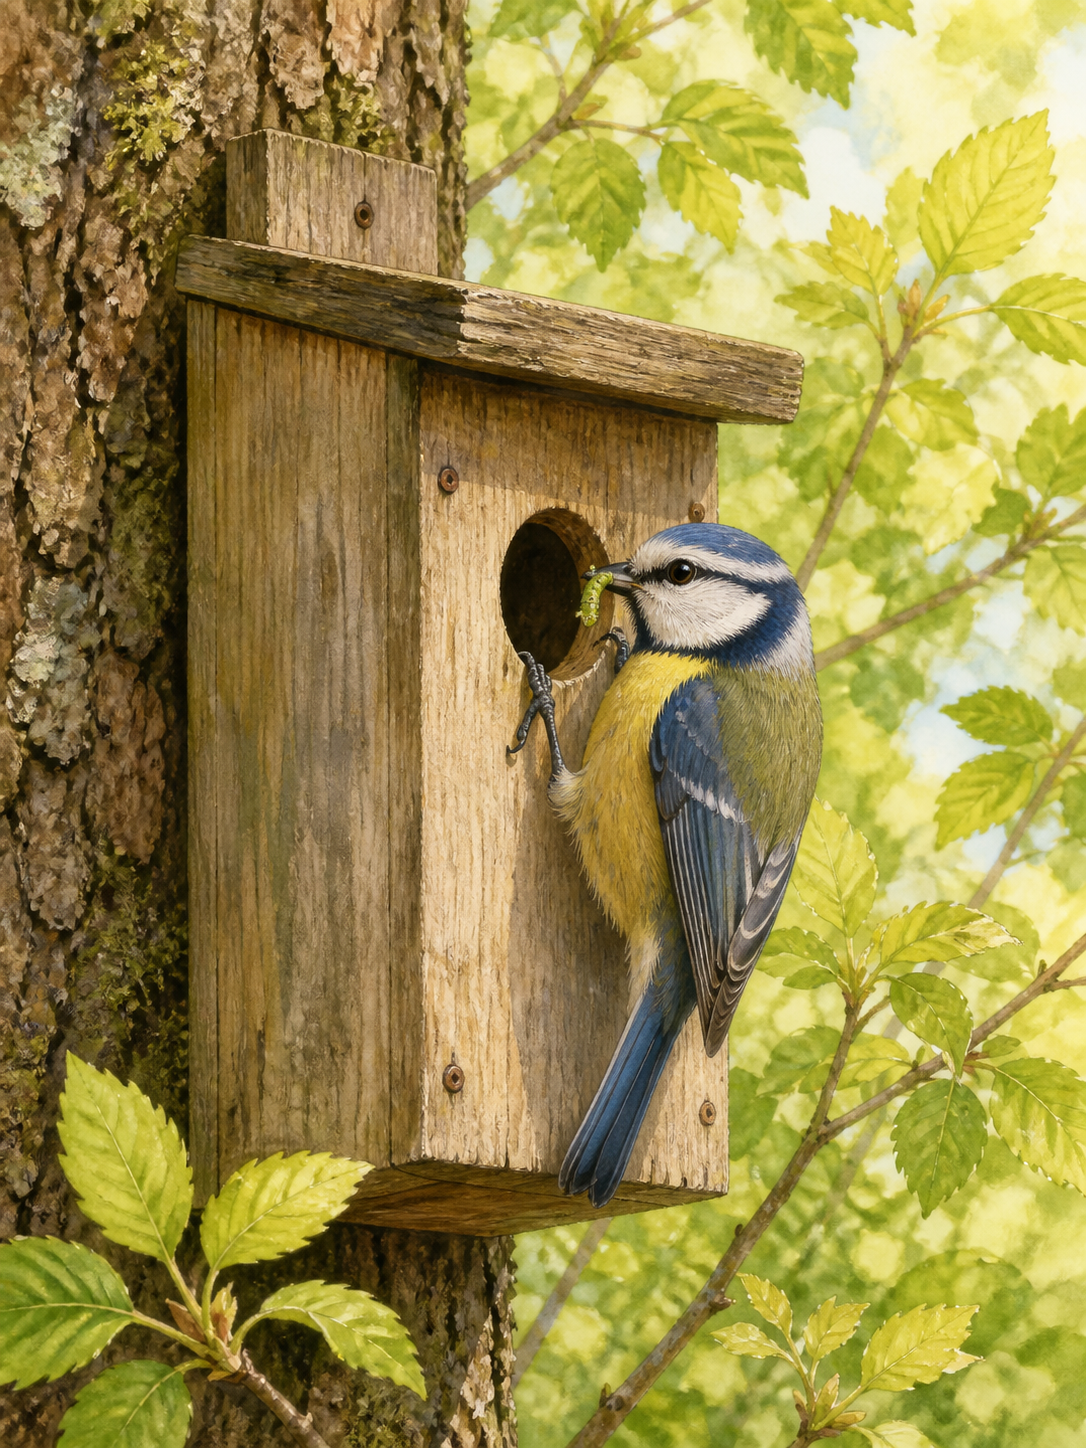
\includegraphics[width=0.46\linewidth]{images/book1/ai/g8-env-nestbox.png}

{\small Calidad del \omterm{def:g2:where-animals-live:habitat}{hábitat}, servida en bandeja: un herrerillo y la
\omterm{ex:g2:animals-grow-up:butterfly}{oruga} a la que estaba ajustada su nidada.}
\end{omfigure}

\begin{example}[Los corderos bajo techo]\label{ex:g8:reproduction-and-environment:lambs}
Los ganaderos de ovejas aprovechan la señal directamente: las ovejas
entran en celo a medida que los días se \emph{acortan}; con una \omterm{def:g6:exploring-our-environment:conditions}{luz}
artificial primero larga y después acortada, un rebaño se puede llevar
a parir para el mercado temprano, que es el rentable. La maquinaria lee
la \omterm{def:g6:exploring-our-environment:conditions}{luz}, no los calendarios --- cambia la \omterm{def:g6:exploring-our-environment:conditions}{luz} y el calendario obedece.
Una señal conocida es una palanca.
\end{example}

\section{Abastecida por el hábitat}

\begin{proposition}[La reproducción se paga en materia]\label{prop:g8:reproduction-and-environment:cost}
Los \omterm{def:g2:animals-grow-up:born}{huevos}, la \omterm{def:g2:animals-grow-up:born}{leche}, el néctar, las \omterm{prop:g3:flowers-fruits-seeds:transform}{semillas} y las astas son todos
\emph{producción} en el sentido de la
\cref{def:g6:matter-from-food:production} --- \omterm{def:g6:plants-are-producers:matter}{materia orgánica} que los
progenitores tienen que conseguir primero. Así que la riqueza del
\omterm{def:g2:where-animals-live:habitat}{hábitat} fija el presupuesto:
\begin{itemize}
  \item una gallina bien alimentada pone a diario; una hambrienta deja
        de poner --- la contabilidad del
        \cref{pb:g6:matter-from-food:1} cuadrando en la línea de los
        \omterm{def:g2:animals-grow-up:born}{huevos};
  \item el haya fructifica en masa solo en los ``años de vecería'', tras
        buenas temporadas de crecimiento --- las cosechas de \omterm{def:g2:from-seed-to-plant:seed}{semilla} son
        veranos ingresados
        (\cref{ex:g6:plants-are-producers:pantry});
  \item los años duros adelgazan la puesta: muchas \omterm{prop:g3:sorting-living-things:groups}{aves} ponen menos
        \omterm{def:g2:animals-grow-up:born}{huevos}, o ninguno, cuando escasean las presas.
\end{itemize}
\end{proposition}
\admitted

\begin{example}[Contar la nidada de los herrerillos]\label{ex:g8:reproduction-and-environment:clutch}
Los estudios con cajas nido enseñan que las nidadas de herrerillo
siguen al suministro de \omterm{ex:g2:animals-grow-up:butterfly}{orugas}: en robledales ricos, diez \omterm{def:g2:animals-grow-up:born}{huevos} o
más; en jardines pobres, seis o siete. El pájaro no decide esto con una
contabilidad --- lo que fija cuánto puede abastecer es el estado de su
cuerpo, construido con la comida del \omterm{def:g2:where-animals-live:habitat}{hábitat}. El tamaño de la nidada es
la calidad del \omterm{def:g2:where-animals-live:habitat}{hábitat}, escrita en \omterm{def:g2:animals-grow-up:born}{huevos}.
\end{example}

\section{Limitada por el mundo: las poblaciones}

\begin{definition}[Población]\label{def:g8:reproduction-and-environment:population}
Una \emph{población}\index{población} son todos los individuos de una
\omterm{def:g5:biodiversity:species}{especie} que viven en un sitio --- las ranas de la charca, las hayas del
bosque. La reproducción le suma; las muertes y las marchas le restan; y
el \omterm{def:g6:exploring-our-environment:components}{entorno} le pone el techo.
\end{definition}

\begin{proposition}[Por qué no explotan las poblaciones]\label{prop:g8:reproduction-and-environment:limits}
Todas las \omterm{def:g5:biodiversity:species}{especies} producen de más --- miles de \omterm{def:g2:animals-grow-up:born}{huevos} por pareja de
ranas, miles de \omterm{prop:g3:flowers-fruits-seeds:transform}{semillas} por haya
(\cref{prop:g4:animal-reproduction:strategies}) --- y sin embargo las
charcas no están macizas de ranas. El excedente se gasta contra los
frenos del \omterm{def:g6:exploring-our-environment:components}{entorno}:
\begin{itemize}
  \item la \emph{depredación} --- las garzas y las larvas de libélula
        del \cref{ex:g4:animal-reproduction:pondcount};
  \item la \emph{comida y el espacio} --- solo hay tantas \omterm{ex:g2:animals-grow-up:butterfly}{orugas},
        tantos agujeros para nidos, tantas manchas de \omterm{def:g6:exploring-our-environment:conditions}{luz} en el \omterm{def:g6:decomposers-and-soil:soil}{suelo}
        del bosque;
  \item las \emph{\omterm{def:g6:exploring-our-environment:conditions}{condiciones}} --- una helada tardía sobre las \omterm{def:g3:flowers-fruits-seeds:parts}{flores}
        (\cref{exo:g3:flowers-fruits-seeds:9}), la sequía sobre la
        charca que encoge de los \omterm{ex:g2:animals-grow-up:frog}{renacuajos}.
\end{itemize}
Por término medio, en un \omterm{def:g2:where-animals-live:habitat}{hábitat} estable, cada pareja se sustituye a sí
misma --- el equilibrio de la \cref{prop:g5:food-webs:balance}, visto
desde el lado de los progenitores.
\end{proposition}
\admitted

\begin{example}[Dos primaveras en la charca]\label{ex:g8:reproduction-and-environment:twosprings}
Primavera 1, suave y lluviosa: agua alta, \omterm{prop:g3:sorting-living-things:groups}{insectos} tempranos --- miles
de \omterm{def:g2:animals-grow-up:born}{huevos}, cientos de ranitas, la \omterm{def:g8:reproduction-and-environment:population}{población} sube. Primavera 2, con
sequía: la charca se reduce a un charco, los \omterm{ex:g2:animals-grow-up:frog}{renacuajos} se hacinan, el
\omterm{def:g7:what-is-respiration:respiration}{oxígeno} baja (\cref{prop:g7:oxygen-in-the-water:drains}), las garzas se
dan un banquete con el banco concentrado --- un puñado de ranitas. Las
mismas ranas, el mismo mecanismo, dos veredictos: el \omterm{def:g6:exploring-our-environment:components}{entorno} refrenda
todas las generaciones.
\end{example}

\begin{remark}[Las personas mueven los frenos]\label{rem:g8:reproduction-and-environment:humans}
Casi todos los efectos humanos sobre la fauna pasan por estos frenos y
no por el mecanismo del \omterm{def:g6:cell-unit-of-life:parts}{núcleo}: las charcas desecadas y los setos
arrancados quitan \omterm{def:g2:where-animals-live:habitat}{hábitat} de cría
(\cref{prop:g2:where-animals-live:loss}); los plaguicidas vacían el
máximo de \omterm{ex:g2:animals-grow-up:butterfly}{orugas} para el que se ajustaron los herrerillos; y las cajas
nido de los jardines y los prados húmedos restaurados del
\cref{ex:g5:biodiversity:storks} devuelven techo. Proteger una \omterm{def:g5:biodiversity:species}{especie}
en la práctica significa proteger el \omterm{def:g6:exploring-our-environment:components}{entorno} al que está enchufada su
reproducción --- señal, presupuesto y frenos a la vez.
\end{remark}

\begin{method}[Auditar un cambio de población]\label{met:g8:reproduction-and-environment:audit}
Cuando una \omterm{def:g8:reproduction-and-environment:population}{población} sube o baja, audita por orden:
\begin{enumerate}
  \item la \emph{sincronización}: ¿siguen coincidiendo la señal y el
        máximo del recurso? (una primavera demasiado temprana puede
        dejar tirados a los pollos después de las \omterm{ex:g2:animals-grow-up:butterfly}{orugas});
  \item el \emph{presupuesto}: ¿cuánto dejó abastecer a los
        progenitores el \omterm{def:g2:where-animals-live:habitat}{hábitat} de esa temporada?
  \item los \emph{frenos}: ¿cuál cambió --- depredadores, comida,
        espacio, \omterm{def:g6:exploring-our-environment:conditions}{condiciones}?
  \item el \emph{\omterm{def:g2:where-animals-live:habitat}{hábitat}}: ¿se ganó o se perdió terreno de cría?
\end{enumerate}
\end{method}

\section{Ejercicios}

\begin{exercise}[$\star$]\label{exo:g8:reproduction-and-environment:1}
¿Por qué pone el herrerillo cuando pone? Nombra la regla y la señal.
\end{exercise}

\begin{exercise}[$\star$]\label{exo:g8:reproduction-and-environment:2}
¿Qué consigue el ciervo con sus fechas de otoño y qué hay que contar?
\end{exercise}

\begin{exercise}[$\star$]\label{exo:g8:reproduction-and-environment:3}
¿Por qué se ``paga en materia'' la reproducción? Da tres pagos de la
\cref{prop:g8:reproduction-and-environment:cost}.
\end{exercise}

\begin{exercise}[$\star$]\label{exo:g8:reproduction-and-environment:4}
¿Qué es una \omterm{def:g8:reproduction-and-environment:population}{población}? ¿Qué suma, qué resta y qué pone el techo?
\end{exercise}

\begin{exercise}[$\star$]\label{exo:g8:reproduction-and-environment:5}
Nombra los tres frenos que gastan el excedente de las ranas.
\end{exercise}

\begin{exercise}[$\star$]\label{exo:g8:reproduction-and-environment:6}
¿Qué informa una nidada de diez \omterm{def:g2:animals-grow-up:born}{huevos} frente a una de seis, y sobre
qué?
\end{exercise}

\begin{exercise}[$\star\star$]\label{exo:g8:reproduction-and-environment:7}
Explica el truco de la \omterm{def:g6:exploring-our-environment:conditions}{luz} de los ganaderos de ovejas y qué demuestra
sobre las señales.
\end{exercise}

\begin{exercise}[$\star\star$]\label{exo:g8:reproduction-and-environment:8}
Vuelve a contar el \cref{ex:g8:reproduction-and-environment:twosprings}
como las cuatro preguntas del
\cref{met:g8:reproduction-and-environment:audit}, respondidas para la
primavera 2.
\end{exercise}

\begin{exercise}[$\star\star$]\label{exo:g8:reproduction-and-environment:9}
Un clima que se calienta adelanta dos semanas a las \omterm{ex:g2:animals-grow-up:butterfly}{orugas} del roble,
pero la señal de duración del día de los herrerillos no cambia. Predice
el desajuste y su línea en la auditoría.
\end{exercise}

\begin{exercise}[$\star\star$]\label{exo:g8:reproduction-and-environment:10}
``Los millones del bacalao no se desperdician --- se gastan''. Defiende
la frase con la \cref{prop:g8:reproduction-and-environment:limits}.
\end{exercise}

\begin{exercise}[$\star\star$]\label{exo:g8:reproduction-and-environment:11}
¿Qué freno mueve cada acción humana: desecar una marisma; colgar cajas
nido; fumigar el huerto contra las \omterm{ex:g2:animals-grow-up:butterfly}{orugas} en mayo; restaurar un prado
húmedo?
\end{exercise}

\begin{exercise}[$\star\star\star$]\label{exo:g8:reproduction-and-environment:12}
Conecta tres capítulos en un párrafo: la línea de estrategias
(\cref{prop:g4:animal-reproduction:strategies}), las pérdidas de la
pirámide (\cref{ex:g6:matter-from-food:pyramid}) y los frenos de este
capítulo --- como una sola explicación de por qué la charca no está
maciza de ranas.
\end{exercise}

\section{Problema: La contabilidad de las cajas nido}

\begin{problem}[{Problema de fin de semana --- diez años de
herrerillos, auditados caja por caja}]\label{pb:g8:reproduction-and-environment:1}
Un colegio hace el seguimiento de veinte cajas nido durante diez años:
fechas de puesta, tamaño de las nidadas y pollos volados por caja ---
junto al registro del tiempo y al diario del jardinero.

\medskip\noindent\textbf{Parte I --- Leer los años normales.}
\begin{enumerate}
  \item Años 1--4: puesta a finales de abril, nidadas de ocho a diez
        \omterm{def:g2:animals-grow-up:born}{huevos} y casi todos los pollos volando. Nombra la señal que
        marca el final de abril y el máximo al que apuntan esas fechas.
  \item Las nidadas del año 3 fueron uno o dos \omterm{def:g2:animals-grow-up:born}{huevos} mayores tras un
        mayo cálido y rico en \omterm{ex:g2:animals-grow-up:butterfly}{orugas} en el año 2 --- los progenitores
        invernaron bien. ¿Qué proposición ilustra esa correlación?
  \item Incluso en los años buenos, alrededor de una quinta parte de
        los \omterm{def:g2:animals-grow-up:born}{huevos} no llega a volar. Enumera los frenos probablemente
        responsables, sacados de la
        \cref{prop:g8:reproduction-and-environment:limits}.
  \item ¿Por qué anota el colegio el tiempo y las labores del jardín
        junto a los \omterm{def:g2:animals-grow-up:born}{huevos}? (Responde con las cuatro preguntas de la
        auditoría.)
\end{enumerate}

\medskip\noindent\textbf{Parte II --- Las anomalías.}
\begin{enumerate}[resume]
  \item Año 5: un marzo cálido y raro sacó las \omterm{ex:g2:animals-grow-up:butterfly}{orugas} dos semanas
        antes; las fechas de puesta apenas se movieron. Predice los
        vuelos del año 5 y nombra la línea que falla en la auditoría.
  \item Año 6: el diario del jardinero anota que se retiraron las \omterm{def:g1:plants-around-us:tree}{ramas}
        muertas de los robles viejos y que la franja de prado se segó
        todos los meses. Los vuelos bajan aunque el tiempo fue bueno.
        ¿Qué líneas de la auditoría implica el diario?
  \item Año 7: se instala una pareja de gavilanes. Las nidadas no
        cambian, pero los recuentos de pollos volados bajan. ¿Qué freno
        se movió y por qué no se movió con él la línea de la
        \emph{nidada}?
  \item Año 8: se duplican las cajas hasta cuarenta; el total de pollos
        volados sube, pero el éxito \emph{por caja} se mantiene igual.
        ¿Qué techo levantaron las cajas nuevas y cuál dejaron intacto?
\end{enumerate}

\medskip\noindent\textbf{Parte III --- El informe.}
\begin{enumerate}[resume]
  \item Escribe la frase de resumen de los diez años que relaciona el
        tamaño de la nidada con la calidad del \omterm{def:g2:where-animals-live:habitat}{hábitat}, citando el
        \cref{ex:g8:reproduction-and-environment:clutch}.
  \item El ayuntamiento propone talar la hilera de robles para hacer un
        aparcamiento y ``compensarlo'' con cincuenta cajas nido más.
        Audita la oferta: ¿cuál de las cuatro cosas --- señal,
        presupuesto, frenos y \omterm{def:g2:where-animals-live:habitat}{hábitat} --- sustituyen las cajas y cuál
        solo la dan los robles?
  \item Recomienda dos medidas de jardinería para el año 11, cada una
        atada a su línea de la auditoría.
  \item Cierra con la moraleja del capítulo en una frase: además de dos
        progenitores, ¿qué necesita cada pollo que vuela?
\end{enumerate}
\end{problem}
